
\begin{frame}[ctb!]
  \frametitle{FCS History}

  \begin{columns}[t]

    \column{.33\textwidth}
    \begin{block}{Spreadsheets}
      \begin{itemize}
        \item very inextensible
        \item basic output
        \item little to no decision making
      \end{itemize}
    \end{block}

    \pause

    \column{.33\textwidth}
    \begin{block}{Simulation Dynamics}
      \begin{itemize}
        \item limited extensibility
        \item aggregate mass flows
        \item limited \textit{in situ} decision making
        \item fleet based
      \end{itemize}
    \end{block}

    \pause

    \column{.33\textwidth}
    \begin{block}{Next Generation FCS}
      \begin{itemize}
        \item extensible
        \item \textit{in situ} decision making
        \item isotopic-based dynamics
        \item facility-level effects
        \item region-level effects
      \end{itemize}
    \end{block}

  \end{columns}
  
\end{frame}

\begin{frame}[ctb!]
  \frametitle{Issues with Current SD Implementations}
  
  \begin{itemize}
    \item fleet-based models lack facility-level detail (e.g., facility
      disruptions, facility location, transportation, etc.)
    \item aggregate mass flows lack isotopic-level detail
    \item static facility (fleet) connections
    \item equation-based model limits simulation extensibility
    \item little-to-no recycled fuel matching fidelity
  \end{itemize}

\end{frame}

\begin{frame}[ctb!]
  \frametitle{Basic \Cyclus Approach}

  \begin{itemize}
    \item treat facilities individually
    \item facilities discretely transact materials
    \item materials are defined by both an isotopic \textit{quality} and
      quantity
    \item designed with extensibility in mind
  \end{itemize}

\end{frame}

\begin{frame}[ctb!]
  \frametitle{Making \Cyclus Extensible}
  
  Instead of treating facilities and materials (i.e., commodities) explicitly,
  leading to less extensibility, \Cyclus treats them generally. Facilities are
  black boxes.
  
  \begin{figure}
    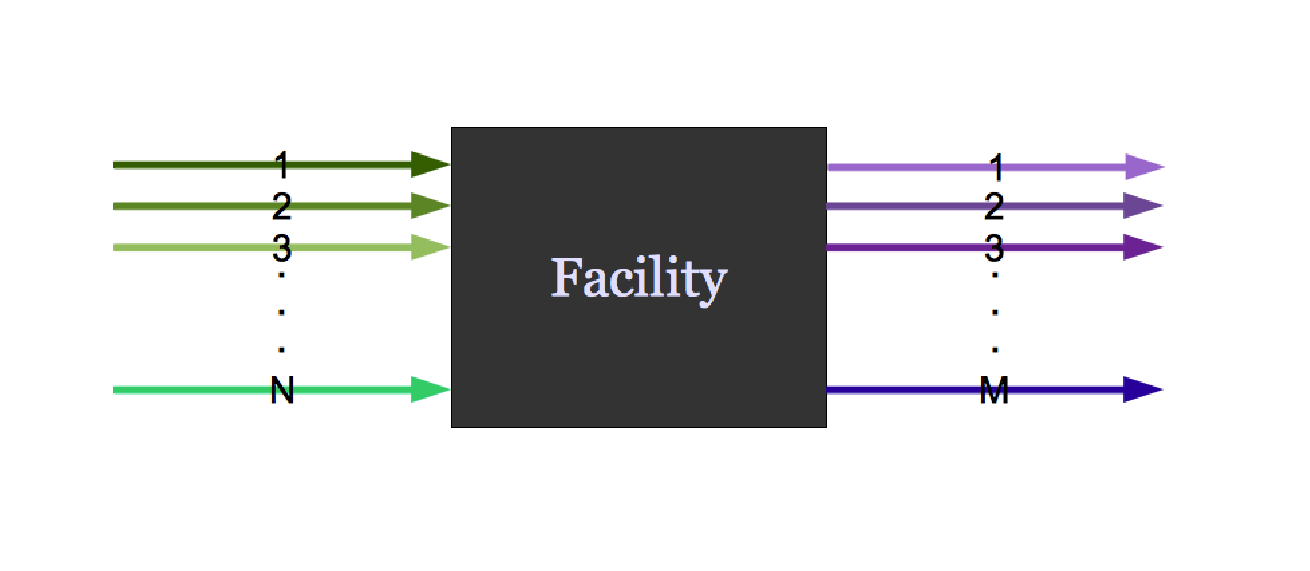
\includegraphics[height=5cm]{./images/facs.eps}
    \caption{Facilities as black boxes. \cite{cyclus2012}.}
    \label{fig:facs}  
  \end{figure}

\end{frame}

\begin{frame}[ctb!]
  \frametitle{Two Motivating Questions}

  \begin{block}{Dynamic Resource Exchange}
    If facilities are treated as individual black boxes and connections between
    facilities are determined dynamically, how does one match suppliers with
    demanders considering supply constraints and, supply response to
    quality-based demands, and issues of fungibility?
  \end{block}

  \pause

  \begin{block}{Fuel Order Approximation}
    Can one model the interface between separations and recycled fuel
    fabrication more realistically?
  \end{block}

\end{frame}
